\iffalse
{Oliver Kopp, Marcel~Kr\"uger, Marei~Peischl}
{Tutorial: Creation of \LaTeX\ documents using a cloud-based pipeline}
{This will be a tutorial on using git as well as GitHub\slash GitLab
pipelines for \LaTeX\ document development. The duration is expected to
be two hours or more, depending on the final schedule.

Most \LaTeX{} users compile on the local machine or using online
services like Overleaf. There also is a third option: build servers.
That option is especially interesting when one versions the project
using git. This tutorial will show you how to get from an installation
of git to a \LaTeX\ document compiled by a build server. At first,
concepts of git and GitHub\slash GitLab will be explained. This includes
the concept of branches, pushes, automated checks on the build server,
and collaborative work using pull\slash merge requests. After that,
there will be time for practical exercises and questions.

Participants are asked to create a GitHub or GitLab account before the
start, but we will also show how to run a pipeline locally so this is
not a strict requirement.}
\fi

\documentclass[final]{ltugboat}
\def\ldots{\tubdots\allowbreak}
\PassOptionsToPackage{draft}{minted}
\usepackage{minted}
\usepackage{xcolor}
\usepackage{microtype}
\usepackage{graphicx}
\usepackage[hidelinks,pdfa]{hyperref}
\usepackage[autostyle]{csquotes}
\usepackage{ragged2e}


\usepackage[bibstyle=tugboat]{biblatex}
\addbibresource{tug2024-cicd.bib}

\usepackage{tabularx}
\usepackage{booktabs}
%%% Start of metadata %%%

\title{Creation of \LaTeX{} documents using a cloud-based pipeline}
\date{2024-07-19}

% repeat info for each author; comment out items that don't apply.
\author{Marei Peischl}
\address{Gneisenaustr. 18\\20253 Hamburg\\Germany}
\netaddress{marei (at) peitex dot de}
\personalURL{https://peitex.de}
%\ORCID{0}
% To receive a physical copy of the TUGboat issue, please include the
% mailing address we should use, as a comment if you prefer it not be printed.
\author{Marcel Krüger}
\address{Hamburg, Germany}
% No printed copy
\EDITORnonetaddress
%\netaddress{marei (at) peitex dot de}
%\personalURL{https://peitex.de}
\author{Oliver Kopp}
\address{Sindelfingen, Germany}
% No printed copy
\EDITORnonetaddress
%\personalURL{https://peitex.de}
\ORCID{0000-0001-6962-4290}


\newif\ifTUGboatPrint

\TUGboatPrinttrue

%black & white mode for printing
\ifTUGboatPrint
\usemintedstyle{bw}
\AtBeginEnvironment{minted}{\let\textit\textsl\let\itshape\slshape}
\AtBeginEnvironment{tcolorbox}{\let\textit\textsl\let\itshape\slshape}
%These are the background colors of the boxes
\colorlet{CommentColBack}{black!2}
\colorlet{ListingColBack}{black!8}
\colorlet{TextColBack}{black!4}
\colorlet{TitleColBack}{white}
\newenvironment{tugboatlisting}[2][]{\VerbatimEnvironment
   	\begin{minted@colorbg}{ListingColBack}\begin{minted}[#1]{#2}}
{\end{minted}\end{minted@colorbg}}


\makeatletter
\renewenvironment{minted@snugshade*}[1]{%
  \def\FrameCommand##1{\hskip\@totalleftmargin
    \colorbox{#1}{##1}\llap{\raisebox{.5ex}[0pt][0pt]{\listingIcon\hspace*{1ex}}}
    %
    \hskip-\linewidth \hskip-\@totalleftmargin \hskip\columnwidth}%
  \MakeFramed{\advance\hsize-\width
    \@totalleftmargin\z@ \linewidth\hsize
    \advance\labelsep\fboxsep
    \@setminipage}%
 }{\par\unskip\@minipagefalse\endMakeFramed}

\makeatother
\newcommand*{\setListingIcon}[1]{\def\listingIcon{#1}}
\setListingIcon{}

\AddToHook{cmd/inputminted/before}{\begin{minted@colorbg}{ListingColBack}}
\AddToHook{cmd/inputminted/after}{\end{minted@colorbg}}
\fi

\usepackage{hologo}
\expandafter\def\csname HoLogo@TeX Live\endcsname{
	\TeX\,Live
}

\usepackage{xspace}




\usepackage{fontspec}

\directlua{luaotfload.add_fallback
("emojifallback",
	{"NotoColorEmoji:mode=harf"}
)}

\setmonofont{Latin Modern Mono}[RawFeature={fallback=emojifallback}]

\newcommand*{\action}[1]{\texttt{#1}}
\newcommand*{\command}[1]{\texttt{#1}}
\newcommand*{\directive}[1]{\textbf{\detokenize{#1}}}
\newcommand*{\file}[1]{\texttt{#1}}
\newcommand*{\directory}[1]{\texttt{#1}}
\newcommand*{\containerimage}[1]{\enquote{#1}}
\newcommand*{\TeXLive}{\acro{\TeX\,Live}\xspace}
\newcommand*{\DEPP}{\acro{DEPP}\xspace}


\usepackage{fontawesome5}

\NewDocumentCommand{\GitHub}{s}{%
	\faIcon{github}%
}
\NewDocumentCommand{\GitLab}{s}{%
	\faIcon{gitlab}%
}
\NewDocumentCommand{\Forgejo}{s}{%
	
\includegraphics[height=1.3\ht\strutbox, alt={Black and white version of the Forgejo Icon}]{forgejo-icon}%
}

\AtBeginDocument{
	\newlength{\mintednumbersep}
	\sbox0{\tiny00}%
	\setlength\mintednumbersep{1em}%
	\addtolength\mintednumbersep{-\wd0}%
	\setminted{numbersep=\mintednumbersep}
}

\setminted{xleftmargin=1em,numbers=left,breakaftersymbolpre={},bgcolor=ListingColBack}
\fvset{fontsize=\small}

\graphicspath{{}{img/}}

\begin{document}



\maketitle


\begin{abstract}
Using web-based platforms for collaborative editing of \LaTeX{} documents is common these days.
These tools focus on writing documents and not on creation of templates or packages.
Using build servers with automated pipelines is common within software development but can easily be adapted for \TeX{} \& Friends.

This article will show how to get started using automated workflows on platforms like GitHub, GitLab or Forgejo for document authors as well as \TeX{} developers.
\end{abstract}

\section{Introduction}
Everything went into or is moving towards the cloud.
\LaTeX{} is already there for about 10 years and today it's quite common to use a web editor for collaboration and local compilation became the \enquote{nerdy} way.
But there also is a third variant to compile documents which can be used also to improve package development and in general the stability of \LaTeX:
adapting DevOps methods, like continuous integration and delivery (\acro{CI/CD}) using automated workflows.

As a very rough working definition, let us consider a \acro{CI/CD} workflow as a number of steps to compile a \TeX{} document to \acro{PDF} on some kind of online service that has access to the source files.

\section{Why continuous integration?}
Having an established workflow usually makes people avoid thinking about changing anything.
So there have to be reasons why it might be worth reading this article or even integrating the mechanisms into projects.

Early adopters of continuous integration techniques in the \TeX{} ecosystems tried to follow the current state of OpenSource development and open a door for contributors in the development process.
For example, the \LaTeX{} Project is currently creating a lot of user interaction via their GitHub projects~\cite{latex3-github} and also takes contributions from which the whole \TeX/\LaTeX{} community will profit.

But the advantages of these methods extend beyond that. We will focus on some cherry-picked aspects of that as the remainder could probably make an article by itself.

\subsection{Works for me?!}
Sometimes, I can successfully compile my document on my machine, but my supervisor can't on their own.
There are tons of reasons why a \TeX{} compilation may succeed on one system and fail on another.
Running some external continuous integration pipeline will not only illustrate the necessary steps to go from source to the full \acro{PDF}.
It will also help understand if problems are machine specific issues or general ones.

\subsection{Compatibility and regression testing}
It is possible to run workflows on multiple \TeX{} distributions or versions.
This can be used to test if there are any issues with some package update before updating a machine to, e.\,g., install the latest MikTeX updates where downgrading may be complicated.\footnote{That's another issue to address … but a different story.}

Additionally, one can also use it to check backwards compatibility, e.\,g., if one collaborator is using a Debian Stable which is stuck on some outdated version.
As mentioned, the \LaTeX{} Project Team is already using these techniques and even provides functionality for regression testing within their build system \enquote{l3build} \cite{l3build}.

Using this as a package developer enables a general interface to be used for regression testing.
This allows to avoid some of the bugs which otherwise would be published and should be found by a user.
Furthermore, it can be used to avoid inconsistent structures, e.\,g., one of the authors recently found that tons of packages and files within \TeXLive{} do not have a proper version number set within the code.

\section{Structure of this tutorial}

The idea is to introduce readers to the basics of setting up automated workflows on GitLab, GitHub, and Forgejo.

This tutorial mainly addresses two groups of users:

\begin{enumerate}
\item authors focusing on typesetting actual content including those collaborating on a document, and
\item package or template developers who provide their work to be used by the first group.
\end{enumerate}

The second group obviously can also  use workflows of the first, e.\,g., for typesetting documentation.
So developers usually use an extended version of the setup provided for the authors.

As all platforms covered by this article are related to the git version control system, we expect the project to be some kind of git repository.
In case the reader does not yet use git, there is a little bit of information attached to this tutorial.
Using that, it would be possible to use git without even noticing as it is attached to the autosave function of an editor.

Because the \LaTeX{} project is using GitHub, we are going to start with a detailed explanation of GitHub Actions and create a matching setup on the other platforms afterwards.
All workflows are available for customization in the template repositories listed in Table \ref{tab:demo-repos}.
Within this article the listings are marked by Icons to not confuse readers as the platform is switched multiple times to show the differences.
\faGithub{} is used to indicate the listing belongs to Github Actions, whereas \faGitlab{} marks the GitLab CI variant.

\section{Compiling a document in a CI pipeline}

\subsection{First steps with GitHub Actions}
\setListingIcon{\GitHub}

To get started, we need a git repository somehow hosted on GitHub.
It does not have to be a public one.

Thinking of the tasks needed to compile a \LaTeX{} document in any “blank slate” environment, we have to do the following:

\begin{enumerate}
\item Prepare the environment and install a \LaTeX{} distribution.
\item Run \LaTeX{} on the document.
\end{enumerate}
%
\noindent GitHub provides pre-configured actions which are able to combine multiple steps, e.\,g., the latex-action \cite{latex-action}.
This  is starting another container inside the action container to run \command{latexmk}.
However, those actions usually limit the configuration options to simplify the interface.
We are going to elaborate on two variants: Using a container image with a full \TeXLive (this section) and a minimal installation (see Section~\ref{sec:minimize}).

The configuration for an action is done by creating a yaml file within the repositories' subdirectory \file{.github/workflows/hello-world.yml}.
The name may be chosen individually.
The following code snippet shows a minimal configuration:

%\begin{listing}
\inputminted{yaml}{examples/hello-world.yml}
%\caption{ \file{.github/workflows/build.yml} directly using a LaTeX action}
% \label{list:hello-world}
%\end{listing}

\begin{description}
\item[name:] of the workflow.
This is important if a project contains multiple workflows.

\item[on:] This directive indicates conditions under which the workflow will be started.
In this configuration, the jobs will be started on any push, i.\,e., whenever the repository on the server receives an update.

Besides attaching the trigger to some user action it is possible use time-based settings.
For all options it is worth to have a look at the configuration manual \cite{github-actions-ref}.
The default settings differ for all platforms, but even may be specific for a single instance.

\item[jobs] contains a list of jobs to be run one after another.
For example, it is quite common to have one job for compiling a document and another one to make the \acro{PDF} available.
In this example, there is only one job called \enquote{action-test}.

\item[runs-on:] This value corresponds to a runner setup.
Runners are the machines to actually execute the jobs defined in a workflow.
It does not have to be the same server as the one where the repository is hosted.
In this example, \enquote{ubuntu-latest} indicates running on one of the provided runners by GitHub which is based on Ubuntu.
It includes NodeJS and some tooling to simplify the work using predefined actions.
A full list of the readily available runners and detailed description of the images can be found at \cite{github-hosted-runners}.

\item[steps:] This is what the workflow should actually do.
As one can see it is possible to directly enter bash code in there.
This example is only creating some output and therefore should run without any issues.
\end{description}

On GitHub, actions are automatically enabled for new repositories.
When combined with an available runner like we do, it is enough to add a yaml configuration file to the repository to see the effect.
After pushing that configuration, the pipeline will start running on all subsequent pushes.
% Be aware that for repository forks, actions need to be enabled explicitly in the tab \enquote{Actions}. % too specific

The current status of an action, i.e., what step it is currently running or if it already finished, can always be checked having a look at
\meta{repository url}\url{/actions} e.\,g., for the first of our demo repositories, this can be found at
{\DeclareFieldFormat{citeurlpostfix}{\url{#1/actions}}\citefield{workflow-github}[citeurlpostfix]{url}}.

\noindent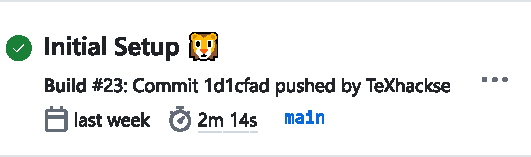
\includegraphics[width=\linewidth,alt={Cropping of a Screenshot from the GitHub Actions status page of a repository. The run was successful. The commit was by @TeXhackse and the commit message says  “Initial setup” followed by a lion emojy.}]{screenshot-pipeline-successful}

The pipeline ran successfully but did not do anything but create some shell output.
Hence, we can move on to the next step: building a \LaTeX{} document.

\subsubsection{Actually using \LaTeX}

Actions are fundamentally based on isolated containers of software, which are run using Docker.
Luckily, some of us live on the Island of \TeX{} and maintain images we could make use of here.\footnote{Special thanks to the other islanders at that point!}
The setup of the images was described within~\cite{islandoftex-docker-short}.

The first part of the workflow will stay the same for the moment.
Changes only apply after \directive{runs-on}:

% This is a stripped down variant of https://github.com/islandoftex/tug2024-workflow-document-github/blob/main/.github/workflows/main.yaml#L63
% Olly thinks, it is OK to keep like that. Line numbers are consistent to the hello-world.yml above.
\inputminted[firstline=5, lastline=12,gobble=3]{yaml}{examples/latex-basic.yml}


\begin{description}
\item[container:] Choosing the IoT \containerimage{texlive-latest} image which provides a full \TeXLive{} + some tools\cite{islandoftex-docker}.
\item[steps:]
The first step looks different from the one, we had before.
It received a name, which is helpful to simplify debugging as GitHub will tell us which step failed.

\item[uses:] is a reference to another action and GitHub's way to reference pre-configured pipelines encapsulating more complex tasks.
In the example, \action{checkout@v4} refers to a separate repository\cite{github-action-checkout}.
This action takes care of the authentication and some internals, so we do not have to deal with details.

The important part is that only after this action, the following steps start being executed within the root directory of our repository.

The second step is kind of the same as in the first example, but this time we run \command{latexmk}~\cite{latexmk} using \command{lualatex}.
By default, this will run on all \file{*.tex} files within the root directory.
So we do not even have to depend on the file name as long as we store files to be included within subdirectories.
\end{description}

\subsubsection{Where is the PDF?}
If the pipeline succeeds, there will be a green checkmark, but we will fail to find the PDF somewhere.
This is because GitHub does not know which (output) files the user actually wants to see or download.
Such files are called \enquote{artifacts}, so now we will adjust the action to keep the PDF and upload it to GitHub as an artifact.

% This is a stream-lined variant from https://github.com/islandoftex/tug2024-workflow-document-github/blob/main/.github/workflows/main.yaml#L48
\inputminted[firstline=13, lastline=17,gobble=5]{yaml}{examples/latex-basic.yml}

After another (successful) run of the pipeline, it is possible to access the \acro{PDF} wrapped within a \file{*.zip} at the run's status page.
Clicking on the run on the actions overview page leads there:

\noindent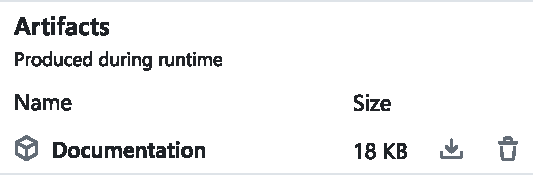
\includegraphics[width=\linewidth,alt={Cropping of a screenshot. It shows the GitHub artifacts download section. A Packaged artifact called “Documentation” is available.}]{screenshot-artifacts}

Sadly, GitHub currently does not provide an option for individual files without a zip.
Also it is not possible to have a static link pointing to the latest artifacts.
Other platforms such as GitLab do provide that feature by default.
To resolve this and make the \acro{PDF} easier to access on GitHub, it is required to use additional actions.
The most common way to do it is publishing the \acro{PDF} to an orphan branch.
Usually this mechanism is used to create web pages and is called \enquote{github-pages}.

To be able to write in the repository, it is necessary to adjust the permissions.
GitHub is providing an interface within the yaml configuration:

\begin{tugboatlisting}[firstnumber=8]{yaml}
permissions:
  contents: write
\end{tugboatlisting}

This has to be added to the job which should upload the pdf.
Additionally, most actions which can be used for uploading artifacts to separate branches request a directory instead of a file.
Consequently, all files have to be moved to a separate directory to be used with these actions.

% This gets added via https://github.com/islandoftex/tug2024-workflow-document-github/pull/1
% (However, the code below is a simplified version)
\begin{tugboatlisting}[breaklines,firstnumber=15]{yaml}
- name: move pdf
   run: mkdir -p build && mv *.pdf build/.
- uses: crazy-max/ghaction-github-pages@v4
  with:
    target_branch: pdf-output
    build_dir: build
  env:
    GITHUB_TOKEN: ${{ secrets.GITHUB_TOKEN }}
\end{tugboatlisting}

The GitHub token also is necessary to be used for the authentication.
Otherwise, the run might be successful, but no PDF will appear on the branch.
%During the preparation of the workshow and this article we've been testing a lot of the uploading actions.
%Actually all somehow do the same, there are just differences in how to configure.

\subsection{Differences to Forgejo Actions}
Forgejo~\cite{forgejo} is another code platform which has the aim to be more open than GitHub.
It can be self-hosted and now provides mechanism similar to GitHub Actions.
They will never act in the same way as GitHub's mechanism, but are almost compatible.

By default, Forgejo searches \directory{.forgejo/workflows/} for configuration files.
If none are found it will even fall back to look inside the \directory{.github/} directory.
The only issue you would probably face from just reusing a GitHub setup is that there are no hosted runners on most instances.
Even if there are runners available, they will probably be different from GitHub's.

However, in case you can configure a runner yourself and use the same labels as the GitHub runner uses (described in~\cite{forgejo-runner-config}), it is possible to use the same workflow configurations on both.
The provided demo repositories on codeberg.org, which is a Forgejo instance, also explain how the runners used there are configured.
% TODO: link to codeberg?

\subsection{Compiling a document using GitLab CI}
\setListingIcon{\GitLab}

GitLab CI is not that much different from the previous Actions setups.
Actually, it is a bit easier to set up continuous integration here as some steps run automatically.
For example, it is not necessary to checkout the repository, because this is already done by default.

The configuration file has to be placed within the repository's root directory and is named \file{.gitlab-ci.yml}.

\inputminted[breaklines,breakafter=/]{yaml}{examples/latex-basic-gitlab.yml}

Here the steps only are a list of commands run after each other. Currently, the list only contains one \command{latexmk} call.

In contrast to GitHub, GitLab is providing an API which allows creating static links to the artifacts.
Thus, the \file{README.md} of the demo repositories there include a link of the following structure:

\begin{FlushLeft}
\meta{Repository URL}\url{/-/jobs/artifacts/}\meta{branch}\allowbreak\url{/browse?job=}\meta{name of the job}
\end{FlushLeft}

This will list all artifacts attached to the job.
Using the example config on one of the demo projects makes it:

\begin{FlushLeft}
{\DeclareFieldFormat{citeurlpostfix}{\url{#1/-/jobs/artifacts/main/browse?job=run-LaTeX}}\citefield{workflow-document-gitlab}[citeurlpostfix]{url}}
\end{FlushLeft}

\section{Testing with multiple versions or compilers}
\setListingIcon{\GitHub}

We promised one can extend these setups to test using multiple \TeX{} versions or engines.
Different engines are actually straightforward to include by running additional steps with different commands.
Of course, it is alternatively possible to use those in separate actions or even workflow files.
There is no general way to structure those as it always depends on whether to always run everything or save resources by conditional or sequential execution.

To use different versions of \TeXLive{}, the Island of \TeX{} provides historic images of all but the latest \TeXLive release (which is not historic yet anyway).

% This is https://github.com/islandoftex/tug2024-workflow-document-github/blob/main/.github/workflows/main.yaml#L56
%  (only some lines simplified, but line numbers are OK!)
\begin{tugboatlisting}[breaklines,breakafter=/:]{yaml}
test-on-IoT-texlive:
  runs-on: ubuntu-22.04
  strategy:
    matrix:
      image: ["TL2022-historic", "TL2023-historic", "latest"]
  name: "Test on ${{ matrix.image }}"
  container:
    image: texlive/texlive:${{ matrix.image }}
  steps:
\end{tugboatlisting}

\begin{description}
\item[strategy:] this is used to create a loop over elements.
In this case, a variable called \mintinline{yaml}|matrix| containing a list of images is used and the content can be accessed within other parts of the file using \mintinline{yaml}|${{ matrix.image }}|.
Thus, the first run will use TL2022, continue on 2023 and finally run on the latest release.
A full list of the provided images can be found at \cite{islandoftex-docker-gitlab}.
\end{description}

Similarly, on GitLab there is also a matrix feature.
The following example even illustrates how to run multiple engines each on multiple \TeXLive releases:
\setListingIcon{\GitLab}

\begingroup
\fvset{commandchars=\\\{\}}
\let\savetheFancyVerbLine\theFancyVerbLine
\def\codecomment{\hspace*{-2\mintednumbersep}\textnormal{[… contains script + artifacts … ]}}
% This is https://gitlab.com/islandoftex/texmf/tug2024-workflow-document-gitlab/-/blob/main/.gitlab-ci.yml?ref_type=heads
% | Listing line | real line |
% | 1, 2         | 1, 2  |
% | 3            | 3 - 7 |
% | 4-           | 8-11    |
\begin{tugboatlisting}[escapeinside=||,breaklines,breakafter=/]{yaml}
check:
  image: registry.gitlab.com/islandoftex/images/texlive:$TEXLIVE_VERSION
\gdef\theFancyVerbLine{}
\codecomment
\gdef\theFancyVerbLine{\addtocounter{FancyVerbLine}{2}}
  parallel:\global\let\theFancyVerbLine\savetheFancyVerbLine
    matrix:
      - TEXLIVE_VERSION: ['TL2022-historic', 'TL2023-historic', 'latest']
        TEX_ENGINE: ['pdflatex', 'xelatex', 'lualatex']
\end{tugboatlisting}
\endgroup

%\renewcommand{\theFancyVerbLine}{%
%\textcolor{red}{\small
%8.\alph{FancyVerbLine}}}

Here the variable is more like a bash variable but can be used the same way.


\section{Minimize the build container}
\label{sec:minimize}\setListingIcon{}
The previous examples used a full \TeXLive installation to have the most convenient setup.\footnote{Almost: the images we used neither include the documentation nor the source tree of \TeXLive.}
The IoT images even ship all dependencies of additional tools such as arara or minted, which enables that all tools in \TeXLive will work out of the box.

Still, sometimes you will not need all the bells and whistles and there are advantages to smaller build containers.
For instance, downloading more than one gigabyte can take quite some time long.
Or you may only have limited disk space available on the runner server.

Side remark: If you are not looking to reduce the images themselves but the compile time because you are building many documents, have a look at last year's IoT article~\cite{islandoftex-docker}.

Back to minimizing the build environment: the most annoying part here might be to find out which packages are actually needed to compile…

So the Island of \TeX{} proudly presents: \DEPP – The DEPendency Printer for \TeXLive\cite{depp}.\footnote{If you are German, do not be surprised if this tool is more clever than its name suggests.}

As this article should focus on pipelines we won't go into detail on the tool itself but instead show how \DEPP produces a file listing all \TeXLive packages necessary for the build.
For the example projects these look like:

\begingroup
\fvset{commandchars=\\\{\}}
% https://github.com/islandoftex/tug2024-workflow-document-github/blob/main/.github/tl_packages#L7
% Note that we added some more packages manually in front:
%  a) latex binaries <-- this is https://gitlab.com/islandoftex/texmf/depp/-/issues/3
%  b) pdftexcmds <-- This is https://gitlab.com/islandoftex/texmf/depp/-/issues/5
%  c) scheme-minimal
\begin{tugboatlisting}[breaklines,linenos=false,xleftmargin=0pt,escapeinside=||]{text}
# Proudly generated by the Island of TeX's …
blindtext
cm
\textnormal{\ensuremath{\vdots}}
\end{tugboatlisting}
\endgroup

\subsection{GitHub}

On GitHub there are multiple actions installing \TeXLive as a part of the workflow~\cite{marcel-latex-action,teatimeguest-latex-action}.
Using those, it is possible to minimize the container and this will also reduce the build time.

\setListingIcon{\GitHub}
% https://github.com/islandoftex/tug2024-workflow-document-github/pull/1 merged?
% not merged: Streamlined version of https://github.com/islandoftex/tug2024-workflow-document-github/blob/main/.github/workflows/main.yaml#L32
% merged: Add +3 to line numbers
\begin{tugboatlisting}[firstnumber=9]{yaml}
- name: Install TeX Live
    uses: zauguin/install-texlive@v3
    with:
      package_file: .github/tl_packages
\end{tugboatlisting}

This snippet can be used within \directive{steps:} and makes the \directive{container:} directive to be obsolete, so it should be removed.
The \directive{package_file:} is the path to the \DEPP output or some manually created list of packages.

 \subsection{GitLab}

On GitLab the simplified syntax makes running a minimized \TeXLive{} a bit more complex.
The \DEPP repository\cite{depp} is luckily providing a shell script to install a \TeXLive based on the package file.
This can be used in the pipelines to modify the container.
Another option would be to provide a container image which already contains the necessary packages.
If a self-hosted runner is used, this usually is the best option as caching can be configured to control when the container is rebuilt or updated.

\section{Pipelines for package developers}

As promised, the advantages of using automated pipelines are even more significant when used within the development process of packages or templates.
In this case, we expect the repository to contain a package and some kind of \command{l3build} configuration.\footnote{Of course, the setup itself also works for other tools, but that is out of scope for this article.}

\subsection{GitHub}\setListingIcon{\GitHub}
The \command{latex} step (calling \command{latexmk} in the examples) is replaced by

% https://github.com/islandoftex/tug2024-workflow-github/blob/main/.github/workflows/main.yaml#L45
\begin{tugboatlisting}[firstnumber=9,breaklines]{yaml}
- name: Run l3build
  run: l3build check --show-log-on-error -q -H
\end{tugboatlisting}

This will automatically run all test files according to the \command{l3build} setup.
As this is within the context of running a package's test suite, the artifacts are totally different.
We are not really interested in a \acro{PDF} but the test output.
One of the authors created another action to take care of this~\cite{marcel-l3build-failure}:

% Streamlined version of https://github.com/islandoftex/tug2024-workflow-github/blob/main/.github/workflows/main.yaml#L47
% (w/o build matrix, w/o comment for the retention days)
\begin{tugboatlisting}[firstnumber=11]{yaml}
- name: Archive failed test output
  if: ${{ always() }}
  uses: zauguin/l3build-failure-artifacts@v1
  with:
    name: testfiles
    retention-days: 3
\end{tugboatlisting}

Apart from uploading the artifacts, this configuration illustrates another important point:
In contrast to the \acro{PDF} of a document, where we are only interested in the success output, we are less interested in success than failure output for test suites.
To let GitHub know that we actually are interested in these artifacts, \mintinline{yaml}|if: ${{ always() }}| has been added.
This will force the step to run also if the previous step failed.

\subsection{GitLab}
\setListingIcon{\GitLab}

Again, GitLab directly supports the artifact upload without loading external extensions.

% https://gitlab.com/islandoftex/texmf/tug2024-workflow-gitlab/-/blob/main/.gitlab-ci.yml?ref_type=heads#L4
\begin{tugboatlisting}[firstnumber=4]{yaml}
  - l3build check --show-log-on-error -q -H
artifacts:
  when: on_failure
  paths:
    - ./build/test/*.diff
\end{tugboatlisting}

This simplifies the standard setup but is less flexible.
For example if you want to use different artifacts for success and failure, it is required to do that within two separate jobs within GitLab.


\section{Running locally}
\setListingIcon{}
Within the tutorial at TUG there was a short journey to running the pipelines locally.
This might be helpful for debugging as one can control the steps manually or to ensure the local setup matches the one on the server.

These setups usually use Docker.
For the platforms which use actions there is a tool called \enquote{act} to simplify that process using the Docker API.
%Forgejo is extending this tool and using it for their runners\cite{forgejo-runner}.

GitLab is extending this by the option to simply have a GitLab runner installed locally.
This provides the option of running

\begin{tugboatlisting}[linenos=false,xleftmargin=0pt]{shell}
gitlab-runner exec
\end{tugboatlisting}

\noindent within a local repository containing some Gitlab CI configuration.

%It's possible to configure the pipelines to run directly on the machine instead of using docker containers.


\section{This is Continuous Development}

Of course every configuration shown here is only an example and can be extended depending on the project's requirements.
It is possible to run arbitrary commands, which might be necessary especially for complex setups.

For example, when creating magazines, it is possible to continuously create a print and an online version, excerpts of single articles as well as HTML/EPUB output, while the editors only have to wait for the compilation of the article they actually are working on.

The same goes for study material where we have rendered version including solutions and some without or documents which share a lot of links between each other and therefore require a lot of runs.

Integrating these structures into more advanced git usage like a useful branching concept can also help to improve collaboration or simplify the contribution process within OpenSource projects.
It will reduce frustration for maintainers as some issues do not have to be checked manually.

\section{Conclusion and Call for Action \& Feedback}
We explained the use of GitHub and GitLab for compiling \LaTeX{} documents and packages.
We showed how different releases of \TeXLive{} and even different compilers can be used to simplify testing across platforms.
Also we  took care of being able to access the PDF or the testing results in some way.

To increase the stability of all parts of \TeX{} development we hope this will help to more tested packages and even less waste of time while compiling complex setups.
In case you maintain some package it would be great if you could now setup some test to check it against the latest version of \TeXLive  or even the current development status.
This can also be a preparation for next years TeX Live pretest, as the Island of \TeX{} also is creating a Docker image for the pretests.
In case you are planning to do that and face any issues, we will try to help.

We would love to maintain this as a tutorial to simplify the use of automation for users of \TeX{} \& Friends.
So if we left open questions, we would love to hear about it and will try to improve this tutorial as well as the examples.

Contributions to this project are very welcome!




\begin{table*}
\caption{Template repositories published with this article. The naming scheme is structured as
\meta{ci-type}\_\meta{task} adding \enquote{\_minimal} if the example is not using a pre-packaged Docker Image but includes methods to install packages based on a dependency file as described in \ref{sec:minimize}. –
All variants listed here have been prepared for at least the 3 platforms mentioned in here.
As the URLs quite long, we published the list including links within the paper's repository {\citefield{tug2024-cicd-tugboat-sources}[citeurl]{url}}.
}
%(github-actions|gitlab-ci|forgejo-actions)-(compile-document|l3build)(-depp)?}
\label{tab:demo-repos}

\ExplSyntaxOn
\cs_set:cpn {latex-Document} {\faCheck}
\cs_set:cpn {latex_testing-Document} {\faCheck}
\cs_set:cpn {l3build-l3build} {\faCheck}
\cs_set:cpn {latex_testing-testing} {\faCheck}
\cs_set:cpn {l3build-testing} {\faCheck}
\begin{tabularx}{\linewidth}{@{}l*{5}{c}@{}}
\toprule
Name& Platforms & Document & l3build & Testing & IoT~Image\\
\midrule
%\clist_map_inline:nn {github-actions, gitlab-ci, forgejo-actions} {
	\clist_map_inline:nn {latex, latex_testing, l3build} {
%		\clist_map_inline:nn {_minimal, \reax} {
			%iot based setups
			#1
			&\faGithub\quad\faGitlab\quad
\includegraphics[height=1.3\ht\strutbox, alt={Black and white version of the Forgejo Icon}]{forgejo-icon}
			&\cs_if_exist_use:c {#1-Document} & \use:c {#1-l3build} & \use:c {#1-testing} &
			\faCheck
			\\
			%minimal setups
			#1_minimal
			&\faGithub\quad\faGitlab\quad
\includegraphics[height=1.3\ht\strutbox, alt={Black and white version of the Forgejo Icon}]{forgejo-icon}
			&\cs_if_exist_use:c {#1-Document} & \use:c {#1-l3build} & \use:c {#1-testing} &
			\\
%		}
	}
%}
\\[-\dimeval{\ht\strutbox+\dp\strutbox}]
\bottomrule
\end{tabularx}
\ExplSyntaxOff
\end{table*}



%\printbibliography
\def\url{\tbsurl}
\SetBibJustification{\raggedright \advance\itemsep by 1pt plus1pt minus1pt }
%\bibliographystyle{tugboat}
%\bibliography{tug2024-cicd}
\printbibliography
\makesignature




\end{document}
